\section{Понятия реляционной теории}
\indent Теория реляционных баз данных оперирует понятиями отношения (relation), от которого и пошло само название теории и баз данных основанных на ней, атрибута, домена, кортежа.

\begin{figure}[ht]
	\centering
	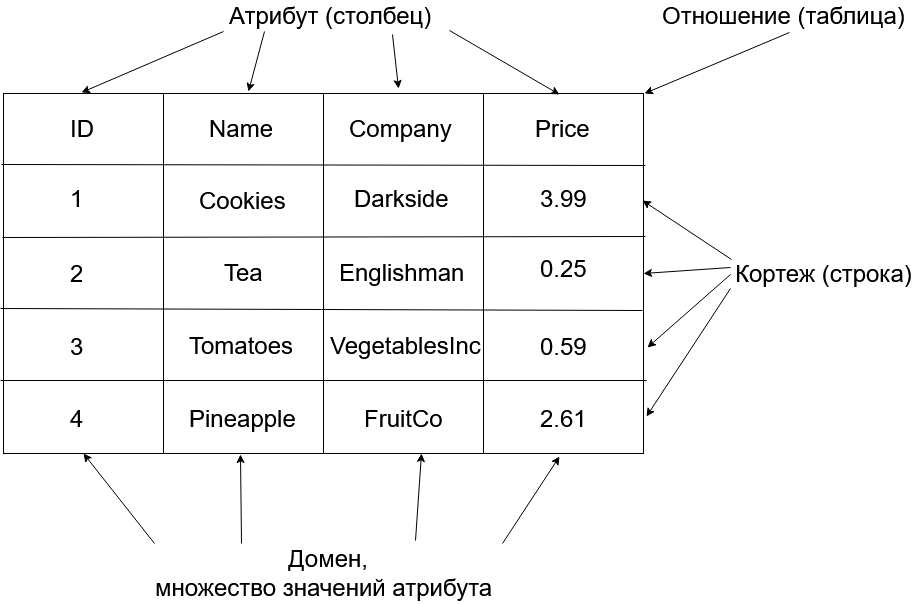
\includegraphics[width=\linewidth]{pics/databaseExample.png}
	\caption{Понятия реляционной базы данных}
	\label{fig:dbExample}
\end{figure}

\indent Атрибут - именованный столбец отношения.
В пределах одного атрибута все значения должны быть одного типа данных, то есть принадлежать одному домену.\\
\indent Домен - тип данных, множество всех допустимых значений атрибута.\\
\indent Кортеж - упорядоченный набор из N элементов, где N - это число атрибутов отношения.
По-другому можно сказать, что кортеж это строка или запись таблицы.\\
\indent Отношение - множество упорядоченных N-кортежей.
Другими словами отношение - это двумерная (плоская) таблица, состоящая из столбцов и строк - атрибутов и кортежей.(см. \ref{fig:dbExample})\\

\todo[inline]{математическое обоснование}
\todo[inline]{полностью переписать, исключить ACID}

\section{Теорема}
\begin{theorem}
	\label{th:th1}
	В любой момент времени можно восстановить необходимую версию карты технологического процесса, при условии того, что вставка в базу данных является атомарным действием, имя искомой карты принадлежит домену "name" отношения "product\_type" и известно значение точки версионирования, которое не меньше заданного в базе данных для карты технологического процесса и меньше следующей точки версионирования.
\end{theorem}

\begin{proof}[Доказательство]
	Используя доказательство от противного, предположим, что нельзя, для любого имени карты из домена "name" отношения "product\_type",восстановить необходимую версию карты технологического процесса, из чего следует утверждение \ref{st:st1}.
	\begin{state}
		\label{st:st1}
		Нельзя создать такой запрос, который, для всех имён карт технологического процесса из домена "name" отношения "product\_types" и любой заданной точки версионирования построит нужную карту.
	\end{state}

	\begin{figure}[ht]
		\centering
		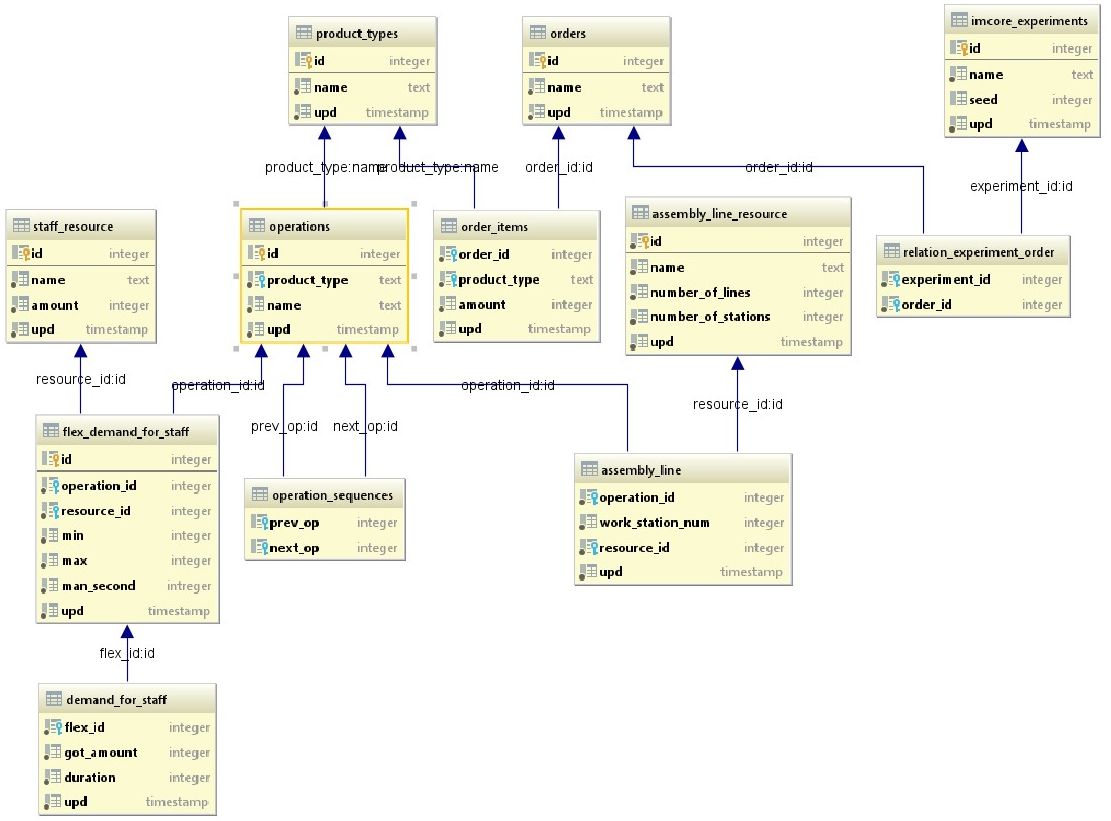
\includegraphics[width=\linewidth]{pics/databaseSchema.png}
		\caption{Схема базы данных}
		\label{fig:dbschema}
	\end{figure}

	\indent Используя схему БД, представленную на рисунке \ref{fig:dbschema}, постараемся доказать обратную теорему.\\
	\indent Введем сокращения названий отношений:

	\begin{itemize}
		\item $product\_types \Rightarrow pr$;
		\item $operations \Rightarrow ops$;
		\item $operation\_sequences \Rightarrow seq$.
	\end{itemize}

	\indent Предположим, есть переменная, принадлежащая домену "name"\ отношения "product\_types"\ $pr\_name \in pr.name$ и переменная $pr\_upd \in \mathbb{Z}$, заданные пользователем, тогда запишем запросы:
	\begin{equation}
		\label{eq:upd}
		pr\_upd" \leftarrow \pi_{pr.upd}(\sigma_{pr.name\ =\ pr\_name\ AND\ pr.upd\ \leq\ pr\_upd}\ pr)
	\end{equation}
	\begin{equation}
		\label{eq:ops}
		ops" \leftarrow \pi_{ops.id,\ pr.name,\ ops.upd}(pr \bowtie_{pr.name = ops.product\_type} ops)
	\end{equation}
	\begin{equation}
		\label{eq:seq}
		seq" \leftarrow \pi_{ops".upd,\ ops".name,\ seq.prev\_op,\ seq.next\_op}(ops" \bowtie_{ops".id = seq.prev\_op} seq)
	\end{equation}
	\begin{equation}
		\label{eq:chart}
		chart \leftarrow \pi_{prev\_op,\ next\_op} (\sigma_{seq".name\ =\ pr\_name\ AND\ seq".upd\ =\ pr\_upd"\ } seq")
	\end{equation}

	\indent Проведем анализ полученных запросов:
	\begin{enumerate}
		\item[1)] в выражении \ref{eq:upd} производится извлечение значения ближайшей (и не большей чем заданная пользователем) точки версионирования;
		\item[2)] затем в выражении \ref{eq:ops} производится объединение отношений "product\_types" и "operations" по атрибуту имени карты технологического процесса, в результате получаем все операции всех карт технологического процесса всех точек версионирования;
		\item[3)] после этого в выражении \ref{eq:seq} объединяются отношение \ref{eq:ops} и "operation\_sequences", что дает все последовательности операций для всех карт технологического процесса всех точек версионирования;
		\item[4)] и в \ref{eq:chart} производится выборка последовательностей из \ref{eq:seq} по имени карты процесса и полученной в выражении \ref{eq:upd} точки версионирования.
	\end{enumerate}

	\indent Так как карта технологического процесса записывается полностью, с одним значением точки версионирования для всех элементов и единовременно, то мы получаем выборку карты, с заданным именем, которое существует в домене "name" отношения "product\_types" и с значением точки версионирования, которая существует в домене "upd" того же отношения и, соответственно, является искомой картой.
	Создание такого запроса опровергает утверждение \ref{st:st1}, а следовательно доказывает теорему \ref{th:th1}.
\end{proof}